% =========================================================================== %
% Scout Installation
% =========================================================================== %

\ifx\wholebook\relax\else
  \documentclass[a4paper,10pt,twoside]{book}
  %=============================================================================%
% Common things, settings, packages to include
%=============================================================================%

\usepackage{graphicx}
\usepackage{color}
\usepackage{makeidx}
\usepackage{ifpdf}
\usepackage{verbatim}

% --------------------------------------------------------------------------- %
% Setting up stuff depeding on output format
% --------------------------------------------------------------------------- %

\ifpdf
  % special settings for pdf mode
  \usepackage[colorlinks]{hyperref}
  \usepackage{courier}
  
  \hypersetup{
    colorlinks,
    linkcolor=darkblue,
    citecolor=darkblue,
    pdftitle={The Eclipse Scout Book},
    pdfauthor={The Scout Community},
    pdfkeywords={Enterprise Framework, Eclipse, Java, Client-Side, Rich Client, Web Client, Mobile},
    pdfsubject={Computer Science}
  }
  
  \usepackage{caption}
  \captionsetup{margin=10pt,font=small,labelfont=bf}
\else
  % special stuff for html mode
  \usepackage[tex4ht]{hyperref}
\fi

% --------------------------------------------------------------------------- %
% Setting up printing range
% --------------------------------------------------------------------------- %

\parindent 1cm
\parskip 0.2cm
\topmargin 0.2cm
\oddsidemargin 1cm
\evensidemargin 0.5cm
\textwidth 15cm
\textheight 21cm

% --------------------------------------------------------------------------- %
% Setting up listings
% --------------------------------------------------------------------------- %

\usepackage{listings}
 
\definecolor{darkviolet}{rgb}{0.5,0,0.4}
\definecolor{darkgreen}{rgb}{0,0.4,0.2} 
\definecolor{darkblue}{rgb}{0.1,0.1,0.9}
\definecolor{darkgrey}{rgb}{0.5,0.5,0.5}
\definecolor{lightblue}{rgb}{0.4,0.4,1}
\definecolor{lightgray}{rgb}{0.97,0.97,0.97}

\renewcommand{\lstlistlistingname}{List of Listings}

% general settings
\lstset{
  basicstyle=\small\ttfamily,
  columns=fullflexible,
  breaklines=true,
  breakindent=10pt,
  prebreak=\mbox{{\color{blue}\tiny$\searrow$}},
  postbreak=\mbox{{\color{blue}\tiny$\rightarrow$}},
  showstringspaces=false,
  backgroundcolor=\color{lightgray}
}

% settings for xml files
\lstdefinelanguage{xml}
{
  commentstyle=\color{darkgrey}\upshape,
  morestring=[b]",
  morestring=[s]{>}{<},
  morecomment=[s]{<?}{?>},
  stringstyle=\color{black},
  identifierstyle=\color{darkblue},
  keywordstyle=\color{cyan},
  morekeywords={xmlns,name,point,factory,class}% list your attributes here
}

% settings for ini files
\lstdefinelanguage{ini}
{
  morecomment=[f][\color{darkgrey}\upshape][0]\#, % # is comment iff it's the first char on the line
  stringstyle=\color{black}
}

% default settings (for java files)
\lstset{
  language=Java,
  emphstyle=\color{red}\bfseries,
  keywordstyle=\color{darkviolet}\bfseries,
  commentstyle=\color{darkgreen},
  morecomment=[s][\color{lightblue}]{/**}{*/},
  stringstyle=\color{darkblue},
}

% --------------------------------------------------------------------------- %
% cross reference macros
% --------------------------------------------------------------------------- %
\newcommand{\applabel}[1]{\label{apx:#1}}
\newcommand{\chalabel}[1]{\label{cha:#1}}
\newcommand{\seclabel}[1]{\label{sec:#1}}
\newcommand{\lstlabel}[1]{\label{lst:#1}}
\newcommand{\figlabel}[1]{\label{fig:#1}}
\newcommand{\tablabel}[1]{\label{tab:#1}}

\newcommand{\appref}[1]{Appendix~\ref{apx:#1}}
\newcommand{\charef}[1]{Chapter~\ref{cha:#1}\xspace}
\newcommand{\secref}[1]{Section~\ref{sec:#1}}
\newcommand{\lstref}[1]{Listing~\ref{lst:#1}\xspace}
\newcommand{\figref}[1]{Figure~\ref{fig:#1}\xspace}
\newcommand{\tabref}[1]{Table~\ref{tab:#1}\xspace}

% --------------------------------------------------------------------------- %
% graphics paths
% --------------------------------------------------------------------------- %
\graphicspath{
  {figures/}
  {Introduction/figures/}
}

%=============================================================================%

  \pagestyle{headings}
  \graphicspath{{figures/} {../figures/}}
  \begin{document}
  \sloppy
\fi


% --------------------------------------------------------------------------- %
\chapter{Scout Installation}
\applabel{install_scout}

% --------------------------------------------------------------------------- %
\section{Overview}

This chapter walks you through the installation of Eclipse Scout. 
The installation description (as well as the rest of this book) is written and tested for Eclipse Scout 3.9.
Scout 3.9.0 will be delivered as part of the Eclipse Kepler release train on June 26, 2013.
Detailed information regarding the scheduling of the Kepler release train is provided in the Eclipse
wiki\footnote{Kepler release plan: \url{http://wiki.eclipse.org/Kepler/Simultaneous_Release_Plan}}.

We assume that you have not installed any software relevant for the content of this book.
This is why the Scout installation chapter starts with the installation of the Java Development Kit (JDK).
Consequently, you will have to skip some of the sections depending on your existing setup.

In the text below, installation routines are described separately for Windows, Mac, and Linux.
As Scout applications have been built primarily on the Windows platform in the past, Scout also has the highest maturity level on this platform.

% --------------------------------------------------------------------------- %
\section{Download and Install a JDK}

The first step to install Scout is to have an existing and working installation of a JDK.
It is recommended to go for the most recent download of Java 7.

You may also use Scout with Java 6.
However, be aware that the communicated end of life for Oracles Java 6 is February 
2013\footnote{Java 6 End of Life: \url{http://www.oracle.com/technetwork/java/eol-135779.html}}.
Java 5 is not supported. 
Running Scout on Java 8 is realistic for the 2014 release train of Eclipse.
This guess is based on the following press 
release\footnote{Java SE Roadmap press release: \url{http://www.oracle.com/us/corporate/press/1854982}}.

\subsection{Windows}

On the Windows platform we recommend to install the Oracle JDK 7 togehter with Scout. 
The reason for this recommendation is simple.
Eclipse Scout is officially tested with the Oracle JDK 7 on Windows.

To successfully install the JDK you need to have at least local admin rights.
It is also necessary that you determine your hardware architecture to decide on the correct JDK installer to download. 
The steps to determine if you are using a 32-bit or a 64-bit version of Windows are described at Microsofts support 
site\footnote{Windows 32/64-bit installation: \url{http://support.microsoft.com/kb/827218}}.

After these preparation steps open Oracles official download 
site\footnote{Official JDK 7 download: \url{http://www.oracle.com/technetwork/java/javase/downloads/index.html}}.
There, you click on the big Java download button and you are shown the various \textit{Java SE Development Kit 7 Downloads}.
Then, accept the licence agreement by clicking on the appropriate radio button.
Select the \textit{Windows x64} package when you are running 64-bit Windows as shown in \figref{jdk_download_oracle}.
If you are running a 32-bit Windows installation, go for the \textit{Windows x86} package.
It is also recommended to download the \textit{Java SE 7 Documentation}.
The documentation package is also available from the official download site, located further down under section \textit{Additional Resources}.

\begin{figure}
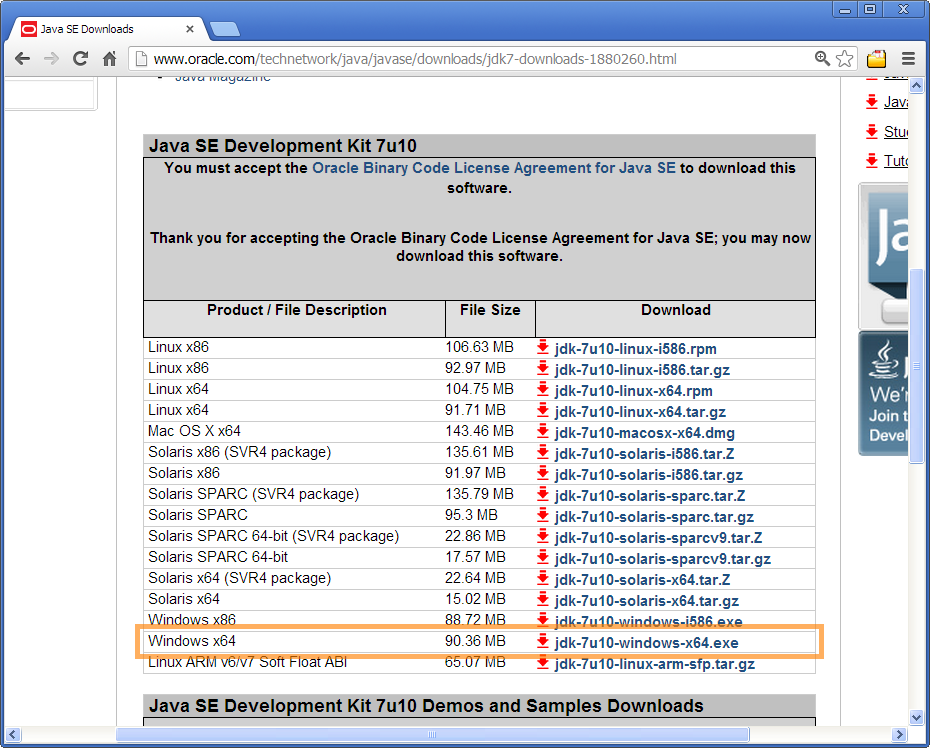
\includegraphics[width=15cm]{oracle_jdk_download.png}
\caption{Installer download for Oracle JDK 7. The Windows 64bit installer package is highlighted.}
\figlabel{jdk_download_oracle}
\end{figure}

Once you have successfully downloaded the JDK installer follow the Windows installation 
guide\footnote{Install the JDK: \url{http://docs.oracle.com/javase/7/docs/webnotes/install/windows/jdk-installation-windows.html\#Run}}.
To verify the installation you might want to go through this Java ''Hello World!'' 
tutorial\footnote{Windows Java ''Hello World!'': \url{http://docs.oracle.com/javase/tutorial/getStarted/cupojava/win32.html}}.

\subsection{Mac}
needs text

\subsection{Linux}
needs text

% --------------------------------------------------------------------------- %
\section{Download and Install Scout}

Installing Eclipse Scout 3.9 requires a working JDK 6 or JDK 7 installation.
If this is missing on your environment, go to the previous section for the necessary installation instructions.

As the Eclipse Kepler release is officially shipped on June 26, 2013 we need to download Scout 3.9 from the developer builds download
page\footnote{Eclipse developer builds download: \url{http://www.eclipse.org/downloads/index-developer.php}}.
The download page should look as shown in \figref{scout_download}.
In this screenshot the packages available for \textit{Eclipse Kepler (4.3) M4} are shown and \textit{Windows} is preselected in the dropdown list.
Should the download page show the wrong platform in the dropdown list, manually fix the selected entry.

\begin{figure}
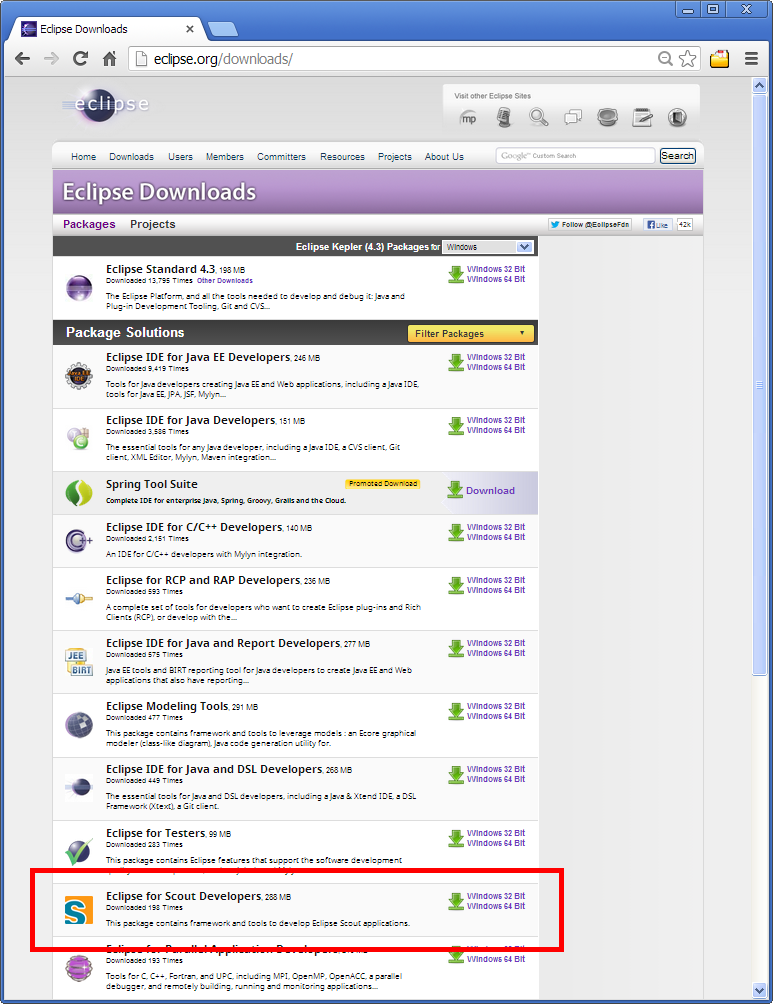
\includegraphics[width=15cm]{scout_download.png}
\caption{Eclipse Kepler developer builds download page. The Scout package is highlighted}
\figlabel{scout_download}
\end{figure}

The following sections describe the installation steps depending on the operating system of your environment.

\subsection{Windows}

For Windows, the Eclipse download page offers two versions for each package.
In \figref{scout_download} the links for these two versions are called \textit{Windows 32 Bit} and \textit{Windows 64 Bit}.
To decide which version to download you first need to know if you have installed a 64-bit JDK or a 32-bit JDK and then download the corresponding Eclipse installation.
Because this is important we are very explicit here: If you are using a 64-bit JDK you must download the 64-bit version of the Eclipse Scout package.
If you are using a 32-bit JDK you must download the 32-bit version of the Eclipse Scout package.
Any other combination will simply not work.

If you just have installed the JDK yourself you will remember what you have installed. 
In case you have a JDK pre-installed you can find out by typing \texttt{java -version} on your console.
For 64-bit JDK installations this fact is explicitly mentioned in the text printed by this command.
The output will then look similar to the text provided below.

\begin{lstlisting}[
  language=console
]
C:\Users\scouty>java -version
java version "1.7.0_02"
Java(TM) SE Runtime Environment (build 1.7.0_02-b13)
Java HotSpot(TM) 64-Bit Server VM (build 22.0-b10, mixed mode)
\end{lstlisting}

If you have installed a 32-bit version this fact is not explicitly mentioned.
See below for an example output of a 32-bit installation.

\begin{lstlisting}[
  language=console
]
C:\Users\scouty>java -version
java version "1.6.0_20"
Java(TM) SE Runtime Environment (build 1.6.0_20-b02)
Java HotSpot(TM) Client VM (build 16.3-b01, mixed mode, sharing)
\end{lstlisting}

With this information you can now correctly choose the version of the Eclipse Scout package to download.
In contrast to the JDK the installation of the Scout package does not require any administrative priviledges.
As the package is a simple ZIP file, you may unpack its content to a location of your choice as shown in \figref{scout_unzip}. 
If possible, we recommend a target directory such as 
\begin{verbatim}
C:\scout\kepler_m4
\end{verbatim}. 
Such a target directory avoids two problems that we had to deal with in the past.
Path names including spaces as well as very long path names that may break the functionality of your zip/unzip tool.

\begin{figure}
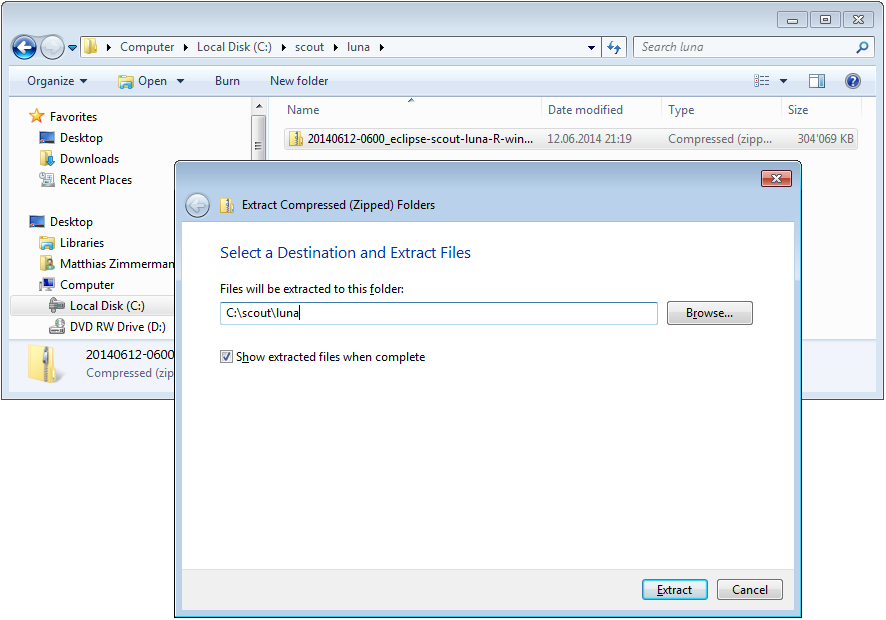
\includegraphics[width=15cm]{scout_extract_zip.png}
\caption{Extracting Eclipse Scout to its target directory}
\figlabel{scout_unzip}
\end{figure}

After unzipping the Scout package, navigate into the subfolder \texttt{Eclipse}.
In case you have installed multiple JDKs coming with their individual Java Runtime Environments (JREs) you might want to explicitly specifiy which JRE to use.
For this, open the file \texttt{eclipse.ini} in a editor of your choice and insert the following two lines at the top of this file
\begin{lstlisting}[
  language=ini
]
-vm
C:\java\jre7\bin\javaw.exe
\end{lstlisting}
where the second line specifies the exact path to the JRE to be used to start your Eclipse Scout installation.
If you have only installed a single JDK you will not need to change the default \texttt{eclipse.ini} file of your Eclipse installation.

\begin{figure}
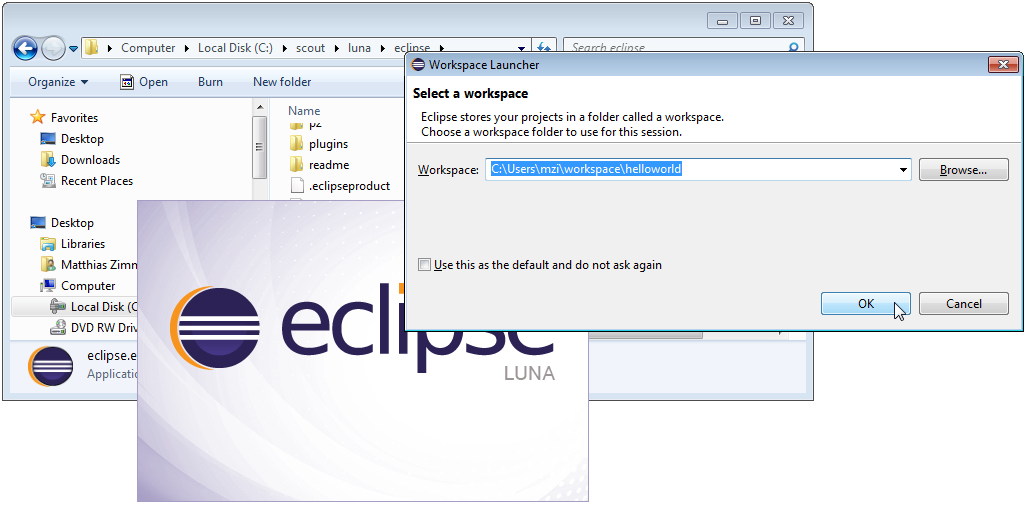
\includegraphics[width=15cm]{scout_startup_select_workspace.png}
\caption{Starting the Eclipse Scout package.}
\figlabel{scout_start}
\end{figure}

You are now ready to start Eclipse Scout via the \texttt{eclipse.exe} file. 
This brings up the workspace launcher as shown in \figref{scout_start}.
Into the \field{Workspace} you enter the target directory of your Scout project.
For a new project you can also enter a path to a directory that does not yet exist.
After clicking the \button{Ok}, Eclipse will create directories that do not yet exist and start the workspace from the specified location.

\begin{figure}
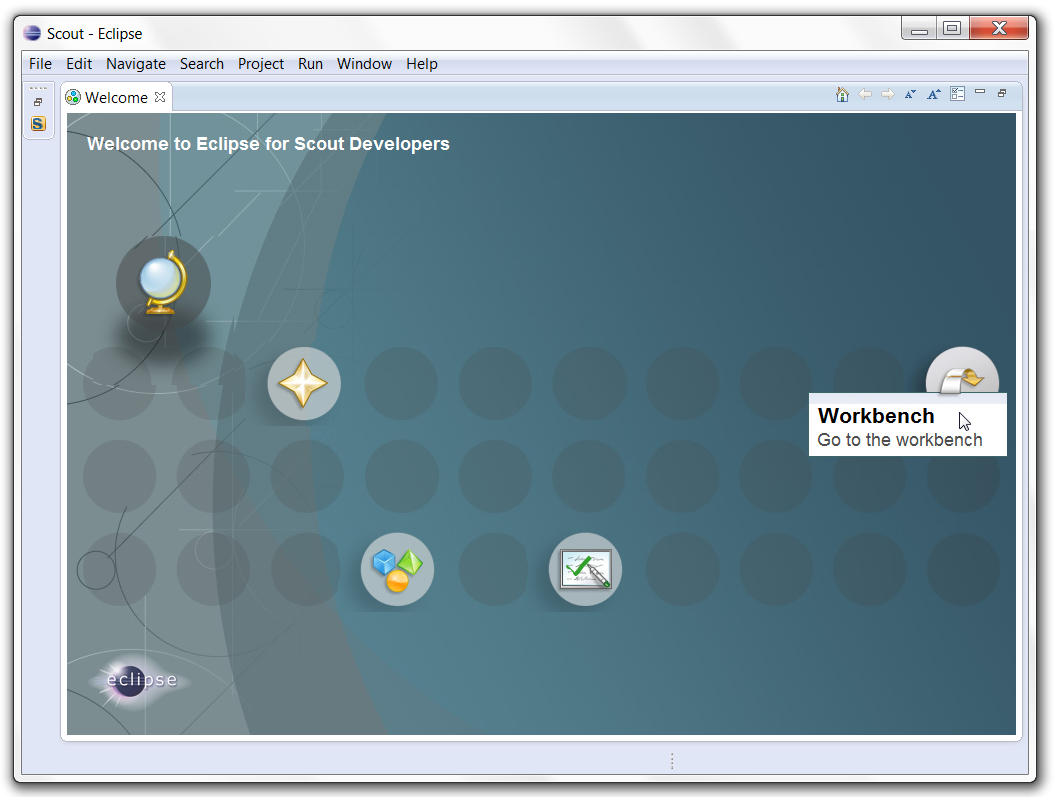
\includegraphics[width=13cm]{scout_startup_welcome.png}
\caption{Eclipse Scout welcome screen.}
\figlabel{scout_welcome}
\end{figure}

\begin{figure}
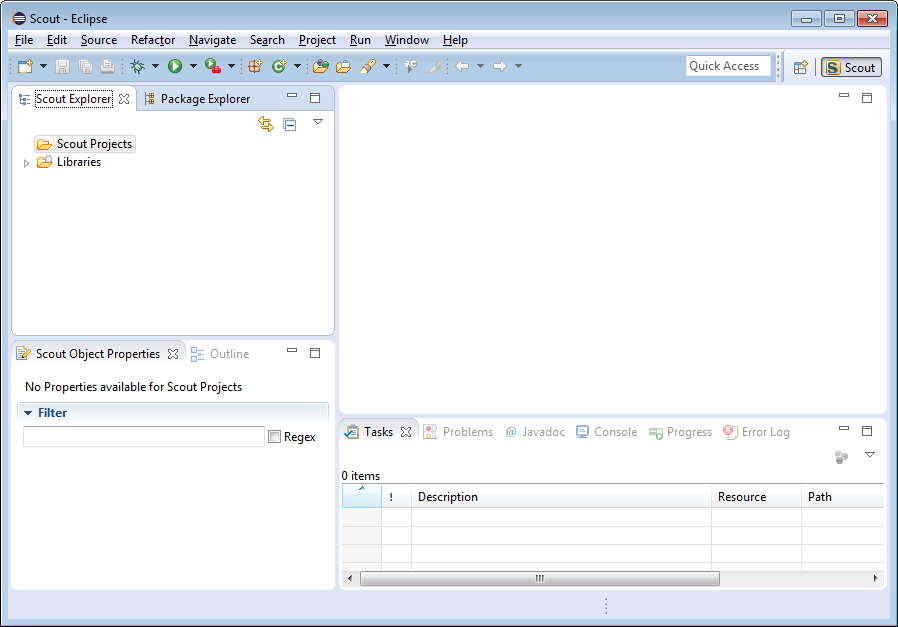
\includegraphics[width=13cm]{scout_startup_scout_explorer.png}
\caption{Eclipse Scout started in the Scout SDK perspective. }
\figlabel{scout_perspective}
\end{figure}

When opening a new workspace for the first time you will be shown the welcome screen as shown in \figref{scout_welcome}.
Click on the \icon{Workbench} to open the Eclipse Scout perspective as shown in \figref{scout_perspective}.

If you have explicitly specified the JRE to be used you verify this in the running Eclipse installation.
Fist, select the \menu{Help|About Eclipse} to open the about dialog.
Then, click on the \button{Installation Details} and switch to the \tab{Configuration}.
In the long list of system properties you will find lines similar to the ones shown below.

\begin{lstlisting}[
  language=ini
]
*** Date: Mittwoch, 9. Januar 2013 20:05:53 Mitteleurop�ische Normalzeit

*** Platform Details:

*** System properties:
...
-vm
C:\java\jre7\bin\javaw.exe
...
sun.java.command=... vm C:\java\jre7\bin\javaw.exe -vmargs ...
\end{lstlisting}

You have now successfully completed the Eclipse Scout installation on your Windows environment.
With this running Scout installation you may skip the following section on how to add Scout to an existing Eclipse installation.

\subsection{Mac}
needs text

\subsection{Linux}
needs text

\fbox{
  \parbox{12cm}{
    \noindent Existing Documentation
    \begin{itemize}
      \item wiki howto \url{http://wiki.eclipse.org/Scout/HowTo/3.8/Install_Scout_SDK}
    \end{itemize}
  }
}
% --------------------------------------------------------------------------- %
\section{Add Scout to your Eclipse Installation}

This section describes the installation of Scout into an existing Eclipse installation.
As the audience of this section is assumed to be familiar with Eclipse, we do not describe how you got your Eclipse installation in the first place.
For the provided screenshots we start from the popular package \textit{Eclipse IDE for Java EE Developers} from the Juno release.

\begin{figure}
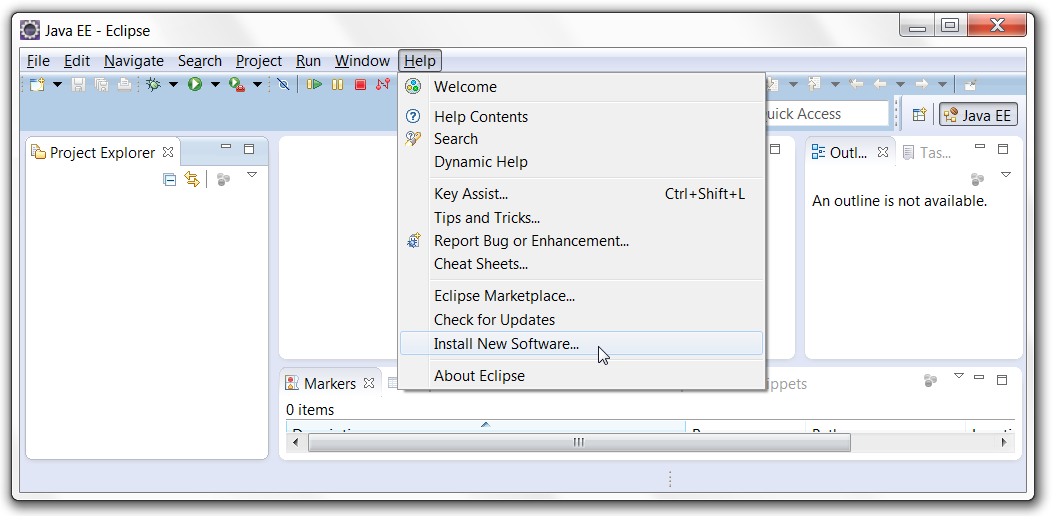
\includegraphics[width=13cm]{eclipse_install_new_software.png}
\caption{Eclipse menu to install additional software}
\figlabel{eclipse_install_new_software}
\end{figure}

To add Scout to your existing Eclipse installation, you need to start Eclipse.
Then select the \menu{Help|Install New Software...} as shown in \figref{eclipse_install_new_software} to open the install dialog.

\begin{figure}
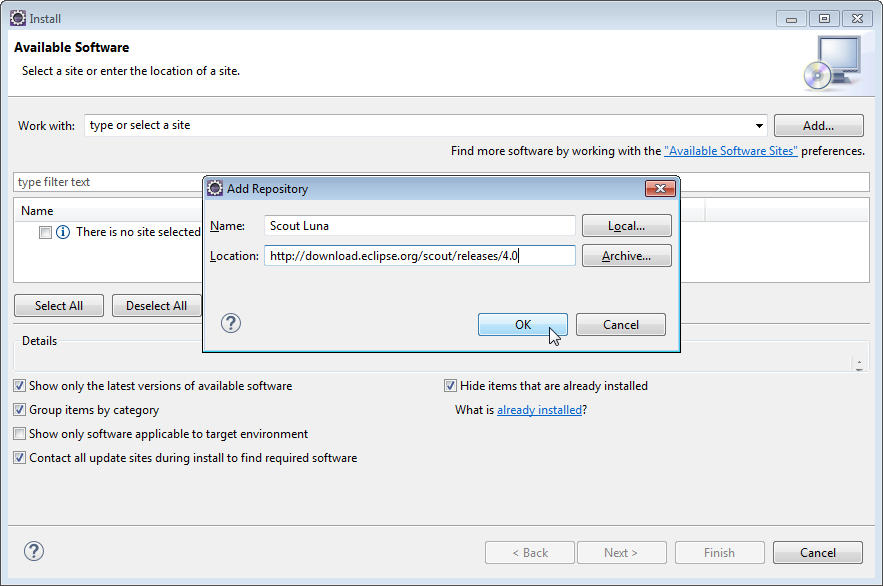
\includegraphics[width=13cm]{eclipse_add_repository.png}
\caption{Add the Scout Kepler repository}
\figlabel{eclipse_add_repository}
\end{figure}

In the install dialog, click on the \button{Add...} to enter the link to the Scout repository.
This opens the popup dialog \textit{Add Repository}
As shown in \figref{eclipse_add_repository} you may use ''Scout Kepler'' for the \field{Name}.
For the \field{Location} enter the Scout Kepler release repository as specified below.
\begin{verbatim}
http://download.eclipse.org/scout/releases/3.9
\end{verbatim}. 

\begin{figure}
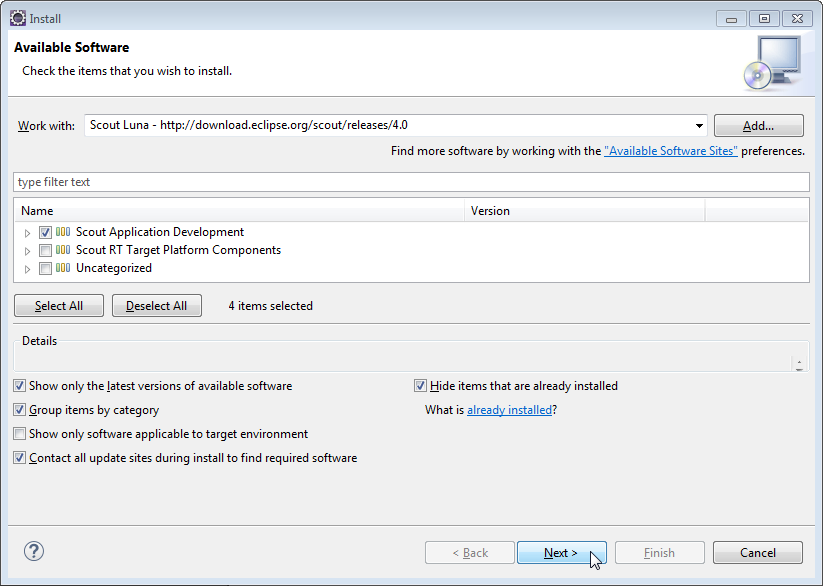
\includegraphics[width=13cm]{eclipse_select_scout_features.png}
\caption{Select the Scout features to add to the Eclipse installation}
\figlabel{eclipse_select_scout_features}
\end{figure}

After connecting to the Scout Kepler repository you may both Scout features as shown in \figref{eclipse_select_scout_features}.
Then, move through the installation with the \button{Next} and accept the presented EPL terms.
Currently, there is still unsigned content included in the features.
So please click away the corresponding warning and accept the request for a restart of Eclipse.
Finally, you may add the Scout perspective to end up at a state very similar to \figref{scout_perspective}.

TODO: Open a bug for this scenario, as a large amount of errors is shown in the \tab{Error Log} of Eclipse.

\fbox{
  \parbox{12cm}{
\noindent Existing Documentation
\begin{itemize}
  \item wiki howto \url{http://wiki.eclipse.org/Scout/HowTo/3.8/Install_Scout_SDK#Add_the_Scout_SDK_to_your_Eclipse_installation}
\end{itemize}
  }
}

% --------------------------------------------------------------------------- %
\section{Verifying the Installation}

The simplest way to verify your Scout installation is to create a ''Hello World'' Scout project and run the corresponding Scout application as described in \charef{helloworld}.

% --------------------------------------------------------------------------- %
\chapter{Further Installations}

% --------------------------------------------------------------------------- %
\section{Download and Install Tomcat}
needs text

\noindent Existing Documentation
\begin{itemize}
  \item wiki tutorial: {http://wiki.eclipse.org/Scout/Tutorial/3.8/Deploy_to_Tomcat}
\end{itemize}

\subsection{Windows}
needs text

\subsection{Mac}
needs text

\subsection{Linux}
needs text

% --------------------------------------------------------------------------- %
\section{Download and Install Jenkins}
needs text

\subsection{Windows}
needs text

\subsection{Mac}
needs text

\subsection{Linux}
needs text

% --------------------------------------------------------------------------- %
\section{Download and Install Maven/Tycho}
needs text

\subsection{Windows}
needs text

\subsection{Mac}
needs text

\subsection{Linux}
needs text

% --------------------------------------------------------------------------- %
\section{Download a Git Client}
needs text

\subsection{Windows}
needs text

\subsection{Mac}
needs text

\subsection{Linux}
needs text

% --------------------------------------------------------------------------- %

\ifx\wholebook\relax\else
   \begin{thebibliography}{99}
  \addcontentsline{toc}{chapter}{Bibliography}
  
  % add/insert books in alphabetical order of 1st author
  
  \bibitem{batessierra05}
    \textit{Bert Bates, Kathy Sierra},
	\textbf{Head First Java} 2nd edition, 
	O'Reilly Media, 2005.

  \bibitem{bloch08} 
    \textit{Joshua Bloch},
    \textbf{Effective Java} 2nd edition, 
	Addison-Wesley, 2008.
	
  \bibitem{eckel06}
    \textit{Bruce Eckel},
	\textbf{Thinking in Java} 4th edition, 
	Prentice Hall International, 2006.

\end{thebibliography}

   \end{document}
\fi

% =========================================================================== %
